\documentclass[11pt,a4paper]{article}
\usepackage[utf8]{inputenc}
\usepackage[T1]{fontenc}
\usepackage{lmodern}
\usepackage[margin=25mm]{geometry}
\usepackage{amsmath,amssymb,mathtools,bm,array,xcolor,booktabs,longtable}
\usepackage{tikz,microtype,enumitem}
\usepackage[nolist]{acronym}
\usetikzlibrary{arrows.meta,positioning,fit}
\usepackage[colorlinks=true,linkcolor=blue!50!black,urlcolor=blue!50!black]{hyperref}
\newenvironment{example}[1]{\par\medskip\noindent\textbf{Worked example: #1.}\ }{\par\medskip}
\setlist[itemize]{noitemsep}
\numberwithin{equation}{section}
\setcounter{tocdepth}{1}

%%%%%%%%%%%%%%%%%%%%%%%%%%%%%%%%%%%%%%%%%%%%%%%%%%%%%%%%%%%%
% MIMO Communications - Common LaTeX Commands
%%%%%%%%%%%%%%%%%%%%%%%%%%%%%%%%%%%%%%%%%%%%%%%%%%%%%%%%%%%%
% Required packages:
% \usepackage{amsmath,amssymb,amsfonts}
% \usepackage{mathtools}
% \usepackage{bm}
% \usepackage{array}
% \usepackage{xcolor}
%
% Convention:
% - Scalars: italic
% - Vectors/matrices: bold lowercase/uppercase
% - Sets: calligraphic
% - Descriptive indices: \mathsf
% - Matrix transpose markers: \mathsf
% - Named mathematical operators: upright
%%%%%%%%%%%%%%%%%%%%%%%%%%%%%%%%%%%%%%%%%%%%%%%%%%%%%%%%%%%%


%%%%%%%%%%%%%%%%%%%%%%%%%%%%%%%%%%%%%%%%%%%%%%%%%%%%%%%%%%%%
% 1. REVIEW AND EDITING
%%%%%%%%%%%%%%%%%%%%%%%%%%%%%%%%%%%%%%%%%%%%%%%%%%%%%%%%%%%%

% Display old text [blue] and proposed text [red]
\newcommand{\Review}[2]{%
	{\color{blue}[#1]}{\color{red}[#2]}}

% Display corrected versions
\newcommand{\Fixed}[2]{%
	{\color{orange}[#1]}{\color{green}[#2]}}

% Show only the accepted version (first argument)
\newcommand{\Done}[2]{#1}

% Comments and notes
\newcommand{\Response}[1]{{\color{magenta}[#1]}}
\newcommand{\Note}[1]{{\color{blue}[#1]}}


%%%%%%%%%%%%%%%%%%%%%%%%%%%%%%%%%%%%%%%%%%%%%%%%%%%%%%%%%%%%
% 2. GENERAL UTILITIES
%%%%%%%%%%%%%%%%%%%%%%%%%%%%%%%%%%%%%%%%%%%%%%%%%%%%%%%%%%%%

% Fixed-width table columns with proper line breaks
\newcolumntype{C}[1]{>{\centering\arraybackslash}p{#1}}
\newcolumntype{R}[1]{>{\raggedleft\arraybackslash}p{#1}}
\newcolumntype{L}[1]{>{\raggedright\arraybackslash}p{#1}}

% Display literal LaTeX text
\newcommand{\ttplain}[1]{\texttt{\detokenize{#1}}}

% Underbraces for expressions in matrices/arrays
\newcommand{\undermat}[2]{%
	\makebox[0pt][l]{$%
		\smash{%
			\underbrace{%
				\phantom{\begin{matrix}#2\end{matrix}}%
			}_{\text{$#1$}}%
		}$}#2}

\newcommand{\coolunder}[2]{%
	\mathrlap{%
		\smash{%
			\underbrace{%
				\phantom{\begin{matrix}#2\end{matrix}}%
			}_{\mbox{$#1$}}%
		}%
	}#2}


%%%%%%%%%%%%%%%%%%%%%%%%%%%%%%%%%%%%%%%%%%%%%%%%%%%%%%%%%%%%
% 3. CROSS-REFERENCING
%%%%%%%%%%%%%%%%%%%%%%%%%%%%%%%%%%%%%%%%%%%%%%%%%%%%%%%%%%%%

\newcommand{\figref}[1]{Figure.~\ref{#1}}
\newcommand{\secref}[1]{Section~\ref{#1}}
\newcommand{\chapref}[1]{Chapter~\ref{#1}}
\newcommand{\theref}[1]{Theorem~\ref{#1}}
\newcommand{\appref}[1]{Appendix~\ref{#1}}
\newcommand{\tabref}[1]{Table~\ref{#1}}

% Define if not already provided by another package
\providecommand{\algref}[1]{}
\renewcommand{\algref}[1]{Algorithm~\ref{#1}}
% Additional packages for notation tables
\usepackage{longtable}
\usepackage{array}
%%%%%%%%%%%%%%%%%%%%%%%%%%%%%%%%%%%%%%%%%%%%%%%%%%%%%%%%%%%%
% 4. MATHEMATICAL OPERATORS AND DELIMITERS
%%%%%%%%%%%%%%%%%%%%%%%%%%%%%%%%%%%%%%%%%%%%%%%%%%%%%%%%%%%%

% Ceiling and floor (mathtools)
\DeclarePairedDelimiter{\ceil}{\lceil}{\rceil}
\DeclarePairedDelimiter{\floor}{\lfloor}{\rfloor}

% Optimization operators
\DeclareMathOperator*{\argmax}{arg\,max}
\DeclareMathOperator*{\argmin}{arg\,min}
\DeclareMathOperator*{\argfirst}{arg\,first}

% Angle/phase of complex quantity
% Overrides any existing \ang definition
\providecommand{\ang}[1]{}
\renewcommand{\ang}[1]{%
	\operatorname{angle}\left(#1\right)}

% Definition symbol
\newcommand{\define}{\triangleq}

% Delimiters (legacy commands)
\newcommand{\LeftP}{\left\lbrace}
\newcommand{\RightP}{\right\rbrace}
\newcommand{\LeftPD}{\left(}
\newcommand{\RightPD}{\right)}

% Additional delimiters
\newcommand{\Abs}[1]{\left|#1\right|}
\newcommand{\inner}[2]{%
	\left\langle #1,#2\right\rangle}


%%%%%%%%%%%%%%%%%%%%%%%%%%%%%%%%%%%%%%%%%%%%%%%%%%%%%%%%%%%%
% 5. SETS AND NUMBER FIELDS
%%%%%%%%%%%%%%%%%%%%%%%%%%%%%%%%%%%%%%%%%%%%%%%%%%%%%%%%%%%%

\newcommand{\compl}{\mathbb{C}}   % Complex field
\newcommand{\real}{\mathbb{R}}    % Real field
\newcommand{\intg}{\mathbb{Z}}    % Integers
\newcommand{\galois}{\mathbb{F}_2} % Binary finite field

% Calligraphic sets
\newcommand{\set}[1]{\mathcal{#1}}


%%%%%%%%%%%%%%%%%%%%%%%%%%%%%%%%%%%%%%%%%%%%%%%%%%%%%%%%%%%%
% 6. VECTORS AND MATRICES
%%%%%%%%%%%%%%%%%%%%%%%%%%%%%%%%%%%%%%%%%%%%%%%%%%%%%%%%%%%%

% Bold lowercase vectors and uppercase matrices
\newcommand{\ma}[1]{\bm{#1}}

% Element indexing
\newcommand{\IndexM}[3]{#1\left[#2,#3\right]}
\newcommand{\IndexV}[2]{#1\left[#2\right]}

% Norms
\newcommand{\Norm}[1]{\left\|#1\right\|}
\newcommand{\NormTwo}[1]{\left\|#1\right\|_2}
\newcommand{\frob}[1]{\left\|#1\right\|_{\mathsf{F}}}

% Matrix operations
\newcommand{\inv}[1]{{#1}^{-1}}
\newcommand{\pinv}[1]{{#1}^{+}}        % Pseudoinverse
\newcommand{\mT}[1]{{#1}^{\mathsf{T}}} % Transpose
\newcommand{\mH}[1]{{#1}^{\mathsf{H}}} % Hermitian transpose
\newcommand{\mC}[1]{{#1}^{*}}         % Complex conjugate

% Matrix properties and functions
\newcommand{\trace}[1]{%
	\operatorname{tr}\left(#1\right)}
\newcommand{\rank}[1]{%
	\operatorname{rank}\left(#1\right)}
\newcommand{\Cond}[1]{%
	\operatorname{cond}\left(#1\right)}
\newcommand{\Det}[1]{%
	\operatorname{det}\left(#1\right)}
\newcommand{\diag}[1]{%
	\operatorname{diag}\left(#1\right)}

% Alias for compatibility
\newcommand{\diagM}[1]{\diag{#1}}

% Vector subspaces
\newcommand{\Span}[1]{%
	\operatorname{span}\left(#1\right)}
\newcommand{\Null}[1]{%
	\operatorname{null}\left(#1\right)}
\newcommand{\Range}[1]{%
	\operatorname{range}\left(#1\right)}

% Vectorization and reshaping
\newcommand{\Vect}[1]{%
	\operatorname{vec}\left(#1\right)}
\newcommand{\unvec}[3]{%
	\operatorname{unvec}_{#2\times #3}\left(#1\right)}

% Matrix products
\newcommand{\elemProd}[2]{#1\odot #2}
\newcommand{\elemDiv}[2]{#1\oslash #2}
\newcommand{\kronProd}[2]{#1\otimes #2}


%%%%%%%%%%%%%%%%%%%%%%%%%%%%%%%%%%%%%%%%%%%%%%%%%%%%%%%%%%%%
% 7. PROBABILITY AND STATISTICS
%%%%%%%%%%%%%%%%%%%%%%%%%%%%%%%%%%%%%%%%%%%%%%%%%%%%%%%%%%%%

% Expectation and variance
\newcommand{\Ex}[1]{%
	\mathbb{E}\left[#1\right]}
\newcommand{\Var}[1]{%
	\operatorname{Var}\left[#1\right]}

% Covariance and correlation
\newcommand{\Cov}[2]{%
	\operatorname{Cov}\left(#1,#2\right)}
\newcommand{\Corr}[2]{%
	\operatorname{Corr}\left(#1,#2\right)}

% Probability of an event
\newcommand{\Prob}[1]{%
	\Pr\left(#1\right)}

% Mean-square error
\newcommand{\MSE}[1]{%
	\operatorname{MSE}\left(#1\right)}

% Distribution notation
\newcommand{\Normal}{\mathcal{N}}
\newcommand{\CNormal}{\mathcal{CN}}

% Complex signal operations
\newcommand{\RE}[1]{%
	\operatorname{Re}\left\{#1\right\}}
\newcommand{\IM}[1]{%
	\operatorname{Im}\left\{#1\right\}}


%%%%%%%%%%%%%%%%%%%%%%%%%%%%%%%%%%%%%%%%%%%%%%%%%%%%%%%%%%%%
% 8. SIGNAL PROCESSING OPERATIONS
%%%%%%%%%%%%%%%%%%%%%%%%%%%%%%%%%%%%%%%%%%%%%%%%%%%%%%%%%%%%

% Fourier transform
\newcommand{\FT}[1]{%
	\mathcal{F}\left\{#1\right\}}

% Circular convolution
\newcommand{\circConv}[2]{#1\circledast #2}

% Modulo reduction notation
\newcommand{\modulo}[2]{%
	\left\langle #1\right\rangle_{#2}}

% Sinc function
\newcommand{\Sinc}[1]{%
	\operatorname{sinc}\left(#1\right)}


%%%%%%%%%%%%%%%%%%%%%%%%%%%%%%%%%%%%%%%%%%%%%%%%%%%%%%%%%%%%
% 9. MIMO DIMENSIONS AND INDICES
%%%%%%%%%%%%%%%%%%%%%%%%%%%%%%%%%%%%%%%%%%%%%%%%%%%%%%%%%%%%

% Subscripts t/r: transmit/receive interfaces
% Superscripts rf/a: RF-chain/antenna-element interfaces
% No superscript: effective digital signal ports
% S: number of data streams
%
% Descriptive indices are upright (\mathsf).
% Running mathematical indices are italic..

% Digital signal ports
\newcommand{\NT}{N_{\mathsf{t}}}
\newcommand{\NR}{N_{\mathsf{r}}}
\newcommand{\nT}{n_{\mathsf{t}}}
\newcommand{\nR}{n_{\mathsf{r}}}

% Data streams
\newcommand{\NS}{S}
\newcommand{\nS}{s}

% RF chains
\newcommand{\NTrf}{N_{\mathsf{t}}^{\mathsf{rf}}}
\newcommand{\NRrf}{N_{\mathsf{r}}^{\mathsf{rf}}}
\newcommand{\nTrf}{n_{\mathsf{t}}^{\mathsf{rf}}}
\newcommand{\nRrf}{n_{\mathsf{r}}^{\mathsf{rf}}}

% Physical antenna elements
\newcommand{\NTa}{N_{\mathsf{t}}^{\mathsf{a}}}
\newcommand{\NRa}{N_{\mathsf{r}}^{\mathsf{a}}}
\newcommand{\nTa}{n_{\mathsf{t}}^{\mathsf{a}}}
\newcommand{\nRa}{n_{\mathsf{r}}^{\mathsf{a}}}


%%%%%%%%%%%%%%%%%%%%%%%%%%%%%%%%%%%%%%%%%%%%%%%%%%%%%%%%%%%%
% 10. MIMO PRECODING AND COMBINING MATRICES
%%%%%%%%%%%%%%%%%%%%%%%%%%%%%%%%%%%%%%%%%%%%%%%%%%%%%%%%%%%%

% Digital precoding and combining
\newcommand{\FD}{\ma{F}_{\mathsf{D}}}
\newcommand{\WD}{\ma{W}_{\mathsf{D}}}

% Analog precoding and combining
\newcommand{\FA}{\ma{F}_{\mathsf{A}}}
\newcommand{\WA}{\ma{W}_{\mathsf{A}}}


% MIMO channel representations

\newcommand{\Ha}{\ma{H}_{\mathsf{a}}}
% Antenna-level channel (physical antenna elements)

\newcommand{\Hrf}{\ma{H}_{\mathsf{rf}}}
% Effective channel after analog TX/RX processing


% H_a: Physical antenna-to-antenna channel
% H_rf: Effective channel between RF-chain interfaces
% H: Effective channel between digital signal ports
% H_s: Effective channel between data streams
%
% H_rf = W_A^H H_a F_A
% H    = W_D^H H_rf F_D
% H_s  = W^H H F


\newcommand{\Hs}{\ma{H}_{\mathsf{s}}}
% Effective stream-level channel after digital
% precoding and combining

% Diversity and multiplexing performance
\providecommand{\odiv}{o_{\mathsf{div}}}   % Diversity order
\providecommand{\gmux}{g_{\mathsf{mux}}}   % Multiplexing gain


%%%%%%%%%%%%%%%%%%%%%%%%%%%%%%%%%%%%%%%%%%%%%%%%%%%%%%%%%%%%
% 11. SIGNAL ENERGY AND NOISE
%%%%%%%%%%%%%%%%%%%%%%%%%%%%%%%%%%%%%%%%%%%%%%%%%%%%%%%%%%%%

\newcommand{\Es}{E_{\mathsf{s}}} % Energy per symbol
\newcommand{\Ed}{E_{\mathsf{d}}} % Total energy

\newcommand{\Eb}{E_{\mathsf{b}}} % Energy per bit

% Noise power spectral density parameter
\newcommand{\Nzero}{N_{0}}

\newcommand{\Ptx}{P_{\mathsf{t}}}
\newcommand{\Prx}{P_{\mathsf{r}}}


%%%%%%%%%%%%%%%%%%%%%%%%%%%%%%%%%%%%%%%%%%%%%%%%%%%%%%%%%%%%
% 12. COMMUNICATION METRICS AND ALGORITHMS
%%%%%%%%%%%%%%%%%%%%%%%%%%%%%%%%%%%%%%%%%%%%%%%%%%%%%%%%%%%%

\newcommand{\SNR}{\mathsf{SNR}}
\newcommand{\SINR}{\mathsf{SINR}}
\newcommand{\CSI}{\mathsf{CSI}}

% Combining and precoding
\newcommand{\MRT}{\mathsf{MRT}}
\newcommand{\MRC}{\mathsf{MRC}}
\newcommand{\ZF}{\mathsf{ZF}}
\newcommand{\LMMSE}{\mathsf{LMMSE}}

% Additional commonly used methods
\newcommand{\LS}{\mathsf{LS}}
\newcommand{\MMSE}{\mathsf{MMSE}}
\newcommand{\ML}{\mathsf{ML}}
\newcommand{\MAP}{\mathsf{MAP}}
\newcommand{\RZF}{\mathsf{RZF}}





%%%%%%%%%%%%%%%%%%%%%%%%%%%%%%%%%%%%%%%%%%%%%%%%%%%%%%%%%%%%
% End of common notation
%%%%%%%%%%%%%%%%%%%%%%%%%%%%%%%%%%%%%%%%%%%%%%%%%%%%%%%%%%%%
\providecommand{\RH}{R_{\ma H}}
\title{MIMO Communications\\Lecture 05: Multiuser MIMO:\\Massive and Distributed MIMO}
\author{Ahmad Nimr}
\date{Winter Semester 2026/27}
\begin{document}
\begin{acronym}
	\acro{p2p}[P2P]{point-to-point}
	\acro{mimo}[MIMO]{multiple-input multiple-output}
	\acro{siso}[SISO]{single-input single-output}
	\acro{simo}[SIMO]{single-input multiple-output}
	\acro{miso}[MISO]{multiple-input single-output}
	\acro{mrc}[MRC]{maximum ratio combining}
	\acro{mrt}[MRT]{maximum ratio transmission}
	\acro{zf}[ZF]{zero forcing}
	\acro{lmmse}[LMMSE]{linear minimum mean-square error}
	\acro{mmse}[MMSE]{minimum mean-square error}
	\acro{svd}[SVD]{singular value decomposition}
	\acro{evd}[EVD]{eigenvalue decomposition}
	\acro{snr}[SNR]{signal-to-noise ratio}
	\acro{sinr}[SINR]{signal-to-interference-plus-noise ratio}
	\acro{csi}[CSI]{channel state information}
	\acro{csir}[CSIR]{channel state information at the receiver}
	\acro{csit}[CSIT]{channel state information at the transmitter}
	\acro{rf}[RF]{radio frequency}
	\acro{qpsk}[QPSK]{quadrature phase-shift keying}
	\acro{awgn}[AWGN]{additive white Gaussian noise}
	\acro{psd}[PSD]{power spectral density}
	\acro{map}[MAP]{maximum a posteriori}
	\acro{mse}[MSE]{mean squared error}
	\acro{ls}[LS]{least squares}
	\acro{ml}[ML]{maximum likelihood }
	\acro{bpsk}[BPSK]{binary phase-shift keying}
	\acro{iid}[IID]{independent and identically distributed}
	\acro{los}[LOS]{line of sight}
	\acro{ostbc}[OSTBC]{orthogonal space-time block code}
	\acro{stbc}[STBC]{space-time block code}
	\acro{dmt}[DMT]{diversity--multiplexing tradeoff}
	\acro{pdf}[PDF]{probability density function}
	\acro{mumimo}[MU-MIMO]{multiuser multiple-input multiple-output}
	\acro{ul}[UL]{uplink}
	\acro{dl}[DL]{downlink}
	\acro{fdma}[FDMA]{frequency-division multiple access}
	\acro{tdma}[TDMA]{time-division multiple access}
	\acro{sdma}[SDMA]{space-division multiple access}
	\acro{bs}[BS]{base station}
	\acro{mac}[MAC]{multiple-access channel}
	\acro{bc}[BC]{broadcast channel}
	\acro{rzf}[RZF]{regularized zero forcing}
	\acro{sic}[SIC]{successive interference cancellation}
	\acro{dpc}[DPC]{dirty-paper coding}
	\acro{dof}[DoF]{degrees of freedom}
	\acro{tdd}[TDD]{time-division duplex}
	\acro{fdd}[FDD]{frequency-division duplex}
	\acro{ap}[AP]{access point}
	\acro{cpu}[CPU]{central processing unit}
	\acro{comp}[CoMP]{coordinated multipoint}
	\acro{cscg}[CSCG]{circularly symmetric complex Gaussian}
	\acro{mu}[MU]{multi-user}
	\acro{se}[SE]{spectral efficiency}
\end{acronym}

\acresetall
\maketitle

\begin{abstract}
	Lecture~04 established linear processing for a given multiuser MIMO channel. This lecture examines how channel properties and system performance scale with the number of base-station ports, user loading, and propagation conditions. The normalized Gram matrix provides a framework for understanding favorable propagation and channel hardening. Representative maximum-ratio and zero-forcing performance and energy-scaling results are derived under explicit channel and CSI assumptions. Pilot overhead, channel estimation errors, and channel aging illustrate practical limitations. Finally, distributed and cell-free architectures extend the same digital MIMO framework to geographically separated access points, highlighting the benefits and challenges of cooperative processing.
\end{abstract}

\acresetall
\tableofcontents
\newpage

% ============================================================


\section{Scaling multiuser MIMO systems}
\label{sec:scaling-05}

\subsection{Learning objectives and connection to Lecture 04}
Lecture~04 established the multiuser signal models, linear combining and precoding methods, and their achievable performance. This lecture examines how these results change with increasing BS port count, user loading, and geographical distribution of the antenna ports. The focus shifts from the processing methods to their statistical behavior, performance scaling, and implementation requirements.

After this lecture, students should be able to distinguish port count from spatial dimensions, interpret normalized channel Gram matrices, explain favorable propagation and channel hardening, assess representative SINR and energy-scaling results, and describe CSI acquisition and distributed MU-MIMO architectures. Both \ac{ul} and \ac{dl} operation are considered, with the main mathematical development based on single-port users and centralized UL reception.

\subsection{Digital model and assumptions}
In the UL, the \ac{bs} receives $U$ independent user signals through $\NR$ effective digital ports:
\begin{equation}
	\boxed{\ma y=\ma H\ma x+\ma v},
	\qquad
	\ma H=[\ma h_1,\ldots,\ma h_U]\in\compl^{\NR\times U}.
	\label{eq:ulmodel-05}
\end{equation}
Here, $\ma y,\ma v\in\compl^{\NR\times1}$, $\ma x\in\compl^{U\times1}$, and $\ma h_u\in\compl^{\NR\times1}$. Independent, zero-mean user symbols satisfy
\begin{equation*}
	\Ex{|x_u|^2}=E_u,
	\qquad
	\ma R_x=\diag{E_1,\ldots,E_U}.
\end{equation*}
The receiver noise is independent of the user signals and assumed \ac{cscg}, with $\ma R_v=\ma C_v=\sigma_v^2\ma I_{\NR}$.

Linear combining gives $\widehat{\ma x}=\mH{\ma W}\ma y$, where $\ma W=[\ma w_1,\ldots,\ma w_U]\in\compl^{\NR\times U}$. The instantaneous user \ac{sinr}, as established in Lecture~04, is
\begin{equation}
	\gamma_u^{\mathsf{UL}}=
	\frac{E_u|\mH{\ma w}_u\ma h_u|^2}
	{\displaystyle\sum_{j\ne u}E_j|\mH{\ma w}_u\ma h_j|^2+
		\sigma_v^2\NormTwo{\ma w_u}^2}.
	\label{eq:ulsinr-05}
\end{equation}
Sections~\ref{sec:statistics-05}--\ref{sec:performance-05} assume perfect instantaneous channel knowledge at the BS and fixed large-scale channel gains. CSI acquisition and estimation errors are considered in Section~\ref{sec:csi-05}. Gaussian signaling is assumed when $\log_2(1+\gamma_u)$ is interpreted as an achievable rate under separate decoding with interference treated as noise.

In the DL, the transpose-based channel convention and common BS energy constraint from Lecture~04 are retained:
\begin{equation*}
	\ma y=\mT{\ma H}_{\mathsf{DL}}\ma F\ma d+\ma v,
	\qquad
	\ma R_d=\Ed\ma I_U,
	\qquad
	\frob{\ma F}^2\leq1,
\end{equation*}
where $\ma H_{\mathsf{DL}},\ma F\in\compl^{\NT\times U}$ and $\ma y,\ma d,\ma v\in\compl^{U\times1}$. The DL SINR depends on the user-channel gains, interuser interference, and the precoder normalization. Unlike the individual UL energy budgets, all DL beams share the BS energy budget $\Ed$. Channel reciprocity and its practical limitations are discussed in Section~\ref{sec:csi-05}.

\subsection{Ports, users, and spatial dimensions}
The number of independent user-channel directions is limited by
\begin{equation*}
	\RH\leq
	\begin{cases}
		\min(\NR,U), & \text{UL},\\
		\min(\NT,U), & \text{DL}.
	\end{cases}
\end{equation*}
Linear ZF separation of all $U$ user streams requires $\RH=U$. This condition is not required for general multiuser communication. In the UL, joint decoding can recover multiple user messages without interference-free linear separation, although the channel rank limits the available spatial degrees of freedom. In the DL, independent receivers generally rely on precoding and interference management, but interference-free ZF is not the only transmission strategy.

A system is underloaded when $U$ is smaller than the number of BS ports, fully loaded when they are equal, and overloaded otherwise. The corresponding loading factors are
\begin{equation*}
	\zeta_{\mathsf{UL}}=\frac{U}{\NR},
	\qquad
	\zeta_{\mathsf{DL}}=\frac{U}{\NT}.
\end{equation*}
These ratios describe dimensional loading but do not determine channel rank or conditioning. Even an underloaded system may have dependent or poorly separated user channels.

Increasing the BS port count for fixed $U$ can improve received signal gain and interference suppression in the UL, or provide additional beamforming and interference-management freedom in the DL. Increasing $U$ for a fixed port count generally increases spatial loading and interuser interference. Joint scaling of ports and users at a fixed loading factor represents a different regime from fixed-user scaling.

Effective digital ports, physical antenna elements, \ac{rf} chains, and active data streams need not have equal counts. A larger physical array therefore does not necessarily provide more independent digital channel directions. Massive MIMO refers to scalable multiuser operation with a large number of BS ports, often substantially exceeding the number of scheduled users, rather than a specific antenna-count threshold or channel distribution. 

\subsection{Normalized channel Gram matrix}
The user-channel interactions introduced in Lecture~04 are described in the UL by the normalized Gram matrix
\begin{equation}
	\ma G_{\NR}=\frac{1}{\NR}\mH{\ma H}\ma H,
	\qquad
	[\ma G_{\NR}]_{ij}
	=\frac{1}{\NR}\mH{\ma h}_i\ma h_j.
	\label{eq:gram-05}
\end{equation}
Its diagonal entries represent normalized channel energies, while the off-diagonal entries describe normalized inner products between different user channels. Their statistical behavior provides the basis for channel hardening and favorable propagation, respectively.

In the DL, the corresponding user-channel Gram matrix is
\begin{equation*}
	\ma G_{\NT}^{\mathsf{DL}}
	=\frac{1}{\NT}\mT{\ma H}\ma H^*.
\end{equation*}
It describes the same geometric properties relevant to beamforming and interuser interference. Under reciprocal propagation with matching calibrated digital ports, the UL and DL channel matrices are related, and the corresponding Gram matrices contain the same channel-energy and alignment information.

For a nonzero channel matrix, the condition number $\mathsf{cond}_H=\sigma_1/\sigma_{\RH}$ describes the spread of its positive singular values. Since this ratio may remain finite for rank-deficient channels, rank and conditioning must be considered separately when assessing linear user separation.

In the two-user example of Lecture~04, increasing channel alignment reduced the smallest singular value and increased the ZF penalty. Additional ports improve user separation only when their channel responses provide useful independent directions. Replicating dependent channel responses may increase received signal energy but does not create additional independent user-channel directions.


\section{Favorable propagation and channel hardening}
\label{sec:statistics-05}

\subsection{Independent Rayleigh fading as a reference}
Consider independent user channels following
\begin{equation}
	\ma h_u\sim\CNormal(\ma 0,\beta_u\ma I_{\NR}),
	\qquad \beta_u>0,
	\label{eq:rayleigh-05}
\end{equation}
where $\beta_u$ denotes the average channel gain per BS port. The channel entries are independent and identically distributed for each user, while the gains $\beta_u$ are held fixed. As $\NR$ increases, independent channel components are added under the same statistical assumptions. This idealized model does not necessarily represent the behavior of a physically enlarged antenna array.

For a fixed number of users, the law of large numbers, Appendix~\ref{app:lln-05}, gives
\begin{equation}
	\boxed{
		\frac{1}{\NR}\mH{\ma H}\ma H
		\xrightarrow[\NR\to\infty]{\mathrm{a.s.}}
		\diag{\beta_1,\ldots,\beta_U}.
	}
	\label{eq:gramlimit-05}
\end{equation}
Thus, the normalized Gram matrix converges to a diagonal matrix. This result combines two distinct statistical properties: favorable propagation and channel hardening. The limit assumes fixed $U$; joint scaling of users and ports is considered separately in Section~\ref{sec:performance-05}.

\subsection{Favorable propagation: separation of different users}
\textbf{Favorable propagation} refers to the asymptotic orthogonality of different user-channel vectors as the number of BS ports increases. For independent Rayleigh channels and fixed users $i\ne j$,
\begin{equation}
	\frac{1}{\NR}\mH{\ma h}_i\ma h_j
	\xrightarrow[\NR\to\infty]{\mathrm{a.s.}}0,
	\qquad
	\Ex{\left|\frac{1}{\NR}\mH{\ma h}_i\ma h_j\right|^2}
	=\frac{\beta_i\beta_j}{\NR}.
	\label{eq:favorable-05}
\end{equation}
Consequently, the normalized channel alignment $c_{ij}$ defined in Lecture~04 approaches zero. This property enables spatial user separation with reduced relative interuser interference.

With unnormalized \ac{mrc}, the desired squared channel coefficient grows proportionally to $\NR^2$, whereas the mean squared coefficient of each interfering user grows proportionally to $\NR$. Thus, the relative interference decreases for fixed $U$ and user energies, although the aggregate interference also depends on the number of users.

In the DL, favorable propagation similarly benefits \ac{mrt}. With $\ma f_j\propto\ma h_j^*$, the interference coefficient at user $u$ is proportional to $\mT{\ma h}_u\ma h_j^*$. Its relative contribution decreases as the user channels become asymptotically orthogonal, subject to the BS energy allocation and precoder normalization.


\subsection{Channel hardening: concentration of one user's gain}
\textbf{Channel hardening} refers to the reduction of relative channel-gain fluctuations as the number of BS ports increases. Under independent Rayleigh fading, the channel energy is
\begin{equation*}
	\NormTwo{\ma h_u}^2=\sum_{\nR=1}^{\NR}|h_{\nR,u}|^2,
	\qquad h_{\nR,u}\sim\CNormal(0,\beta_u).
\end{equation*}
Each squared magnitude has mean $\beta_u$ and variance $\beta_u^2$. Since the channel entries are independent, the mean and variance of the total channel energy are
\begin{equation}
	\begin{split}
		\Ex{\NormTwo{\ma h_u}^2}
		&=\sum_{\nR=1}^{\NR}\Ex{|h_{n,u}|^2}
		=\NR\beta_u,\\
		\Var{\NormTwo{\ma h_u}^2}
		&=\sum_{n=1}^{\NR}\Var{|h_{\nR,u}|^2}
		=\NR\beta_u^2.
	\end{split}
	\label{eq:channel-moments-05}
\end{equation}
Thus, the normalized channel energy converges to its average gain:
\begin{equation}
	\boxed{
		\frac{\NormTwo{\ma h_u}^2}{\NR}
		\xrightarrow[\NR\to\infty]{\mathrm{a.s.}}\beta_u,
		\qquad
		\frac{\Var{\NormTwo{\ma h_u}^2}}
		{\Ex{\NormTwo{\ma h_u}^2}^2}
		=\frac{1}{\NR}.
	}
	\label{eq:hardening-05}
\end{equation}
The standard deviation of the channel energy grows as $\sqrt{\NR}\beta_u$, whereas its mean grows as $\NR\beta_u$. Consequently, the relative standard deviation decreases as $1/\sqrt{\NR}$. Channel hardening therefore makes the channel energy increasingly predictable relative to its mean, without eliminating the need for channel-direction information in spatial processing. The same result applies to the DL under the corresponding independent Rayleigh model, with $\NT$ replacing $\NR$.

\begin{example}{Relative fluctuations and array size}
	For $\NR=4,16,64$, the relative standard deviation of the channel energy is $0.5,0.25,0.125$, respectively. A fourfold increase in port count halves the relative fluctuations. These results concern small-scale fading with fixed $\beta_u$; changes in path loss or shadowing may still change the average channel gain.
\end{example}

Favorable propagation concerns the separation of different user channels, whereas channel hardening concerns fluctuations in individual channel gains. Neither property implies the other. For example, channels $\ma h_u=\sqrt{\beta_u}e^{j\theta_u}\ma a$, with deterministic $\NormTwo{\ma a}^2=\NR$, have constant energy but are collinear. Conversely, independent random scalar gains multiplying mutually orthogonal deterministic vectors preserve orthogonality without necessarily producing channel hardening.

\subsection{Spatial correlation}
The independent fading model can be generalized to spatially correlated channels. Consider independent, zero-mean \ac{cscg} user channels with
\begin{equation*}
	\ma h_u\sim\CNormal(\ma 0,\ma C_{h_u}),
	\qquad
	\ma C_{h_u}=\Ex{\ma h_u\mH{\ma h}_u}
	\in\compl^{\NR\times\NR}.
\end{equation*}
For these channels, the relative channel-energy variance is
\begin{equation}
	\boxed{
		\frac{\Var{\NormTwo{\ma h_u}^2}}
		{\Ex{\NormTwo{\ma h_u}^2}^2}
		=\frac{\trace{\ma C_{h_u}^2}}
		{\trace{\ma C_{h_u}}^2}.
	}
	\label{eq:corrhard-05}
\end{equation}
For two independent users $i\ne j$, the normalized covariance overlap is
\begin{equation}
	\boxed{
		\frac{\Ex{|\mH{\ma h}_i\ma h_j|^2}}
		{\Ex{\NormTwo{\ma h_i}^2}\Ex{\NormTwo{\ma h_j}^2}}
		=\frac{\trace{\ma C_{h_i}\ma C_{h_j}}}
		{\trace{\ma C_{h_i}}\trace{\ma C_{h_j}}}.
	}
	\label{eq:overlap-05}
\end{equation}
The first ratio measures channel hardening, while the second characterizes statistical overlap between user channels. Both are dimensionless and do not fully characterize the available spatial degrees of freedom. In particular, the second ratio is a ratio of ensemble moments rather than the expected squared instantaneous alignment. Their derivations are provided in Appendix~\ref{app:moments-05}. 

For increasing port count, convergence of the first ratio to zero implies concentration of normalized channel energy, while convergence of the second implies vanishing normalized cross-user coupling in mean square. These conditions depend on the spatial covariance structure, not merely on the number of ports. For the DL, the same expressions apply to the channel-column covariances $\ma C_{h_u}^{\mathsf{DL}}\in\compl^{\NT\times\NT}$.

As an extreme example, consider fully correlated channels
\begin{equation*}
	\ma h_u=g_u\ma a,
	\qquad
	g_u\sim\CNormal(0,\beta_u),
	\qquad
	\NormTwo{\ma a}^2=\NR.
\end{equation*}
The channel covariance is $\ma C_{h_u}=\beta_u\ma a\mH{\ma a}$, giving a relative energy variance of one for every $\NR$. If all users share the same $\ma a$, their channel vectors remain collinear despite independent scalar fading. Increasing the number of ports therefore does not guarantee channel hardening or favorable propagation.


% ============================================================

\section{Massive MIMO performance and scaling}
\label{sec:performance-05}

\subsection{Maximum-ratio combining: instantaneous and statistical SINR}
The \ac{mrc} direction from Lecture~04 is retained. For statistical analysis, the unit-norm combiner $\ma w_u=\ma h_u/\NormTwo{\ma h_u}$ is used without changing the SINR:
\begin{equation}
	\gamma_u^{\mathsf{UL},\MRC}
	=\frac{E_u\NormTwo{\ma h_u}^2}
	{\displaystyle\sum_{j\ne u}E_j
		\frac{|\mH{\ma h}_u\ma h_j|^2}{\NormTwo{\ma h_u}^2}
		+\sigma_v^2}.
	\label{eq:mrcinstant-05}
\end{equation}
Under independent Rayleigh fading, the mean channel energy is $\NR\beta_u$, while each normalized interference projection has mean $\beta_j$. Replacing the numerator and denominator by their respective means gives the  mean-power \ac{sinr} ratio
\begin{equation}
	\boxed{
		\widetilde\gamma_u^{\mathsf{UL},\MRC}
		=\frac{E_u\NR\beta_u}
		{\displaystyle\sum_{j\ne u}E_j\beta_j+\sigma_v^2}.
	}
	\label{eq:mrcproxy-05}
\end{equation}
This mean-power \ac{sinr} ratio  illustrates the dependence on port count, user energies, and large-scale channel gains. It is generally neither the mean instantaneous SINR nor an exact achievable-rate expression. For fixed $U$, the normalized interference projections need not concentrate even as $\NR$ increases. The statistical derivation is provided in Appendix~\ref{app:mrc-05}. 

With fixed user energies and fixed $U$, the desired gain increases with $\NR$, while the interference-plus-noise denominator remains of finite statistical order. The SINR therefore benefits from additional ports, although strong interfering users may still cause substantial interference. User scheduling and energy allocation remain relevant.

\subsection{Zero forcing and excess spatial dimensions}
For a full-column-rank UL channel with $U\leq\NR$, the \ac{zf} SINR from Lecture~04 is
\begin{equation*}
	\gamma_u^{\mathsf{UL},\ZF}
	=\frac{E_u}
	{\sigma_v^2[\inv{(\mH{\ma H}\ma H)}]_{uu}}.
\end{equation*}
Under independent Rayleigh fading, the projection of user $u$ onto the subspace orthogonal to the other $U-1$ user channels has $\NR-U+1$ complex dimensions. The mean ZF SINR is therefore
\begin{equation}
	\boxed{
		\Ex{\gamma_u^{\mathsf{UL},\ZF}}
		=\frac{E_u\beta_u}{\sigma_v^2}(\NR-U+1).
	}
	\label{eq:zfmean-05}
\end{equation}
This result is exact for the independent Rayleigh reference model with perfect CSI and spatially white noise. Increasing the number of excess spatial dimensions reduces the typical ZF penalty. At $\NR=U$, ZF is feasible almost surely but the remaining useful projection has only one complex dimension.

The mean inverse-Gram diagonal is finite only for $\NR>U$, where
\begin{equation*}
	\Ex{[\inv{(\mH{\ma H}\ma H)}]_{uu}}
	=\frac{1}{\beta_u(\NR-U)}.
\end{equation*}
The inverse of this mean is not the mean SINR in \eqref{eq:zfmean-05}. Likewise, the mean SINR does not directly determine the ergodic achievable rate.

The \ac{lmmse} combiner retains its maximum-linear-SINR property from Lecture~04 and therefore achieves an instantaneous SINR no smaller than that of MRC or feasible ZF under the same channel and energy assumptions. Its advantage depends on channel conditioning, user loading, and operating energy. The related DL \ac{rzf} method balances interference suppression and precoder norm under a shared transmit-energy constraint.

\begin{example}{Array size and scheduled users}
	Consider independent Rayleigh fading with $E_u=\beta_u=\sigma_v^2=1$ and perfect CSI. The MRC mean-power \ac{sinr} ratio and exact mean ZF SINR are compared in \tabref{tab:scaling-05}.
	\begin{table}[htbp]
		\centering
		\caption{MRC mean-power SINR ratio and mean ZF SINR
			under independent Rayleigh fading (linear scale).}
		\label{tab:scaling-05}
		\begin{tabular}{rrrr}
			\toprule
			$\NR$ & $U$ &
			$\widetilde\gamma_u^{\mathsf{UL},\MRC}$ &
			$\Ex{\gamma_u^{\mathsf{UL},\ZF}}$\\
			\midrule
			64  & 8  & 8  & 57\\
			64  & 32 & 2  & 33\\
			128 & 8  & 16 & 121\\
			\bottomrule
		\end{tabular}
	\end{table}
	Increasing the port count at fixed $U$ improves both results. Increasing $U$ at fixed port count reduces the available spatial separation resources. The displayed quantities characterize different statistics and must not be interpreted as ergodic rates.
\end{example}

\subsection{Energy scaling and user loading}
Consider fixed $U$, independent Rayleigh fading, perfect CSI, and fixed large-scale gains. If all user energies decrease proportionally to the inverse BS port count,
\begin{equation*}
	E_u=\frac{\mathcal E_u}{\NR},
\end{equation*}
where $\mathcal E_u$ is constant, both MRC and ZF satisfy
\begin{equation}
	\boxed{
		\gamma_u^{\mathsf{UL},\MRC}
		\xrightarrow[\NR\to\infty]{\mathrm p}
		\frac{\mathcal E_u\beta_u}{\sigma_v^2},
		\qquad
		\gamma_u^{\mathsf{UL},\ZF}
		\xrightarrow[\NR\to\infty]{\mathrm p}
		\frac{\mathcal E_u\beta_u}{\sigma_v^2}.
	}
	\label{eq:energyscale-05}
\end{equation}
The increasing array gain compensates the reduced user energy, while the residual interference becomes negligible relative to the output noise. This result assumes perfect CSI independently of the decreasing data energy. Reduced pilot energy may degrade channel estimation and change the scaling.

A different regime arises when the number of users grows with the port count. For equal fixed user energies $E_u=E$, equal large-scale gains $\beta_u=\beta$, and $U/\NR\to\zeta\in(0,1)$,
\begin{equation}
	\widetilde\gamma_u^{\mathsf{UL},\MRC}
	\longrightarrow\frac{1}{\zeta},
	\qquad
	\Ex{\gamma_u^{\mathsf{UL},\ZF}}
	\sim\frac{E\beta}{\sigma_v^2}\NR(1-\zeta).
	\label{eq:jointscaling-05}
\end{equation}
Under this reference model, the actual MRC SINR also converges in probability to $1/\zeta$. Although individual normalized cross-user channel products vanish, the aggregate interference remains significant because the number of interfering users grows with $\NR$. ZF eliminates this interference while retaining a fraction of the available spatial dimensions.

Thus, fixed-user scaling and joint user/port scaling describe different operating regimes. Additional energy-allocation cases are considered in Appendix~\ref{app:extensions-05}.

\subsection{Downlink scaling and spectral efficiency}
The channel statistics also govern DL beamforming, but the BS energy budget is shared among the users. Under the transpose-based DL convention, unit-norm \ac{mrt} beams are
\begin{equation*}
	\ma b_u=\frac{\mC{\ma h}_u}{\NormTwo{\ma h_u}},
	\qquad
	\ma f_u=\sqrt{\alpha_u}\,\ma b_u,
	\qquad
	\sum_{u=1}^{U}\alpha_u\leq1.
\end{equation*}
The desired received energy is $\Ed\alpha_u\NormTwo{\ma h_u}^2$. For independent DL Rayleigh channels \(\mathbf h_u\sim\mathcal{CN}(\mathbf0,\beta_u\mathbf I_{N_{\mathsf t}})\),  with $\ma h_u\in\compl^{\NT\times1}$, the instantaneous DL MRT SINR is
\begin{equation}
	\gamma_u^{\mathsf{DL},\MRT}
	=\frac{\Ed\alpha_u\NormTwo{\ma h_u}^2}
	{\displaystyle\Ed\sum_{j\ne u}\alpha_j
		\frac{|\mT{\ma h}_u\mC{\ma h}_j|^2}
		{\NormTwo{\ma h_j}^2}
		+\sigma_u^2}.
	\label{eq:mrtinstant-05}
\end{equation}
The desired channel energy has mean $\NT\beta_u$, while each normalized interfering projection has mean $\beta_u$. A corresponding ratio-of-means proxy is
\begin{equation}
	\boxed{
		\widetilde\gamma_u^{\mathsf{DL},\MRT}
		=\frac{\Ed\alpha_u\NT\beta_u}
		{\displaystyle\Ed\beta_u\sum_{j\ne u}\alpha_j+\sigma_u^2}.
	}
	\label{eq:mrtproxy-05}
\end{equation}
As in the UL, this mean-power \ac{sinr} ratio illustrates scaling but is not generally the mean SINR or an ergodic-rate expression. For fixed $U$ and energy allocations, increasing $\NT$ provides coherent gain. With equal allocation $\alpha_u=1/U$, increasing the scheduled user count reduces the energy assigned to each beam.

For DL ZF, the interference is eliminated when the user channels are linearly independent. With global normalization from Lecture~04,
\begin{equation*}
	\gamma_u^{\mathsf{DL},\ZF}
	=\frac{\Ed}{\sigma_u^2\frob{\ma B}^2},
	\qquad
	\ma B=\ma H^*\inv{(\mT{\ma H}\ma H^*)}.
\end{equation*}
Under independent Rayleigh fading with equal large-scale gains $\beta$ and sufficiently many excess ports, the typical normalization scales approximately as
\begin{equation*}
	\frob{\ma B}^2
	\approx\frac{U}{\beta(\NT-U)},
	\qquad
	\gamma_u^{\mathsf{DL},\ZF}
	\approx\frac{\Ed\beta(\NT-U)}{U\sigma_u^2}.
\end{equation*}
These expressions describe large-system behavior rather than exact finite-array mean SINRs. The DL ZF gain therefore depends on both the excess spatial dimensions and the number of users sharing the BS energy.

For a specified processing method and Gaussian signaling, the instantaneous user rate is
\begin{equation*}
	R_u(\ma H)=\log_2(1+\gamma_u(\ma H)),
\end{equation*}
with ergodic rate $\overline R_u=\Ex{R_u(\ma H)}$ and sum rate $R_{\mathsf{sum}}=\sum_u R_u$. In general, neither $\log_2(1+\Ex{\gamma_u})$ nor the rate computed from a mean-power SINR ratio equals the ergodic rate. Increasing the number of served users may improve sum spectral efficiency while reducing individual rates, depending on processing, energy allocation, and user-channel conditions.

Finally, reduced radiated energy does not necessarily imply reduced total system energy. Additional ports increase hardware, CSI acquisition, and signal-processing requirements. The net benefit depends on the resulting performance gains and implementation costs.


\section{Channel state information and pilot limitations}
\label{sec:csi-05}

\subsection{Coherence blocks and orthogonal pilots}
The preceding analysis assumes perfect instantaneous \ac{csi}. In practice, channel coefficients must be estimated and used while the channel remains approximately constant. Consider a coherence block containing $M$ complex channel uses, determined by the coherence time and bandwidth. If $M_{\mathsf c}$ uses are allocated to channel estimation, the number of data uses satisfies $M_{\mathsf d}\leq M-M_{\mathsf c}$. These resources may be shared between UL and DL operation.

In the UL, user $u$ transmits a known pilot sequence $\ma\phi_u\in\compl^{M_{\mathsf c}\times1}$ with $\NormTwo{\ma\phi_u}^2=M_{\mathsf c}$ and pilot-symbol energy $E_u^{\mathsf p}$. The received pilot matrix is
\begin{equation}
	\ma Y_{\mathsf p}
	=\sum_{j=1}^{U}\sqrt{E_j^{\mathsf p}}\,
	\ma h_j\mT{\ma\phi}_j+\ma V_{\mathsf p},
	\label{eq:pilotmodel-05}
\end{equation}
where $\ma Y_{\mathsf p},\ma V_{\mathsf p}\in\compl^{\NR\times M_{\mathsf c}}$. The pilot noise is assumed independent \ac{cscg} with variance $\sigma_v^2$ per entry. Correlation with the known pilot gives
\begin{equation}
	\begin{split}
		\ma r_{\mathsf p,u}
		&=\frac{1}{M_{\mathsf c}}\ma Y_{\mathsf p}\mC{\ma\phi}_u\\
		&=\sqrt{E_u^{\mathsf p}}\ma h_u
		+\sum_{j\ne u}\sqrt{E_j^{\mathsf p}}\,
		\ma h_j\frac{\mH{\ma\phi}_u\ma\phi_j}{M_{\mathsf c}}
		+\ma n_u,
	\end{split}
	\label{eq:pilots-05}
\end{equation}
where $\ma r_{\mathsf p,u},\ma n_u\in\compl^{\NR\times1}$ and $\ma R_{n_u}=(\sigma_v^2/M_{\mathsf c})\ma I_{\NR}$. The observation contains the desired channel, interference from nonorthogonal pilots, and receiver noise.

\textbf{Orthogonal pilots} satisfy
\begin{equation}
	\mH{\ma\phi}_i\ma\phi_j=M_{\mathsf c}\delta_{ij}.
	\label{eq:pilotorth-05}
\end{equation}
Thus, contributions from other orthogonally trained users vanish after correlation, yielding $\ma r_{\mathsf p,u}=\sqrt{E_u^{\mathsf p}}\ma h_u+\ma n_u$. Since the pilot space has dimension $M_{\mathsf c}$, at most $M_{\mathsf c}$ mutually orthogonal nonzero sequences can be assigned. Orthogonal training of all $U$ users therefore requires $M_{\mathsf c}\geq U$.

For nonorthogonal or reused pilots, the cross-correlation terms in \eqref{eq:pilots-05} remain. Such interference may arise from simultaneous training of too many users, pilot reuse in neighboring cells, or loss of pilot orthogonality due to synchronization errors and channel variation. Orthogonality removes modeled pilot interference but not receiver noise or other estimation errors.

The total pilot energy of user $u$ is $M_{\mathsf c}E_u^{\mathsf p}$, whereas $E_u$ denotes its data-symbol energy. Increasing $M_{\mathsf c}$ improves the matched observation quality when pilot energy per use is fixed, but reduces the resources available for data. With a fixed total pilot-energy budget, increasing the pilot length alone does not improve the observation SNR under the ideal model.

\begin{example}{Pilot overhead and scheduled users}
	Consider $M=200$ channel uses. For $U=20$, orthogonal pilots require at least $M_{\mathsf c}=20$, leaving at most $M_{\mathsf d}=180$ data uses, or $90\%$ of the block. For $U=80$, the minimum pilot allocation increases to $80$ uses, leaving at most $60\%$ for data. Additional spatially separable users therefore do not necessarily increase the net spectral efficiency.
\end{example}

For a data-phase ergodic rate $\overline R_u^{\mathsf{data}}$, the net spectral efficiency is
\begin{equation}
	\mathrm{SE}_u
	=\frac{M_{\mathsf d}}{M}\overline R_u^{\mathsf{data}}.
	\label{eq:prelog-05}
\end{equation}
The prelog accounts for the available data resources but does not by itself describe estimation errors. The data-phase rate must be evaluated using the actual CSI and decoding assumptions.

\subsection{CSI acquisition in TDD and FDD}
In \ac{tdd}, UL and DL transmissions occupy different time intervals in the same frequency band. Under reciprocal propagation and sufficiently slow channel variation, UL pilot measurements can be reused for DL channel acquisition. With matching antenna ports, the physical UL and DL channel matrices are related by transposition, consistent with the adopted DL convention.

However, the effective digital channels also include transmit and receive hardware responses. RF calibration and knowledge of the frontend processing are therefore required to exploit reciprocity at the digital interfaces. The numbers of effective BS receive and transmit ports may differ, $\NR\ne\NT$, so complete UL and DL digital channel matrices need not have matching dimensions. Only channel components corresponding to common physical ports and known processing mappings can be related. With full reciprocal digital-port coverage, TDD pilot overhead primarily depends on the number of users rather than the BS port count.

In \ac{fdd}, UL and DL operate at different carrier frequencies, so instantaneous channel reciprocity cannot generally replace DL estimation and feedback. The required measurements and feedback may increase with the BS port count. Statistical correlation, channel structure, and compressed feedback can reduce this overhead, but do not eliminate the general CSI acquisition challenge.

\subsection{Imperfect CSI and pilot contamination}
Channel estimation errors affect the combining and precoding methods introduced in Lecture~04. Let the estimated UL channel be
\begin{equation}
	\widehat{\ma H}=\ma H+\ma E,
	\qquad
	\ma E=[\ma e_1,\ldots,\ma e_U]\in\compl^{\NR\times U},
	\label{eq:channelerror-05}
\end{equation}
where $\ma e_u=\widehat{\ma h}_u-\ma h_u$ denotes the estimation error. The combining matrix $\ma W$ is computed from $\widehat{\ma H}$, while the received data depend on the actual channel $\ma H=\widehat{\ma H}-\ma E$. The combined signal becomes
\begin{equation}
	\begin{split}
		\widehat{\ma x}
		&=\mH{\ma W}\ma y\\
		&=\mH{\ma W}\widehat{\ma H}\ma x
		-\mH{\ma W}\ma E\ma x
		+\mH{\ma W}\ma v.
	\end{split}
	\label{eq:imperfectcombining-05}
\end{equation}
The additional term describes the mismatch caused by channel estimation errors. It may affect desired-signal gain and introduce residual interference even when the estimated channels are perfectly separated.

For example, the \ac{mrc} combiner is formed using $\ma w_u=\widehat{\ma h}_u$. The output for user $u$ is
\begin{equation}
	\begin{split}
		\widehat x_u
		={}&\underbrace{\NormTwo{\widehat{\ma h}_u}^2x_u}_{\text{estimated desired signal}}
		+\underbrace{\sum_{j\ne u}
			\mH{\widehat{\ma h}}_u\widehat{\ma h}_j x_j}_{\text{estimated interference}}\\
		&-\underbrace{\sum_{j=1}^{U}
			\mH{\widehat{\ma h}}_u\ma e_jx_j}_{\text{channel estimation error}}
		+\underbrace{\mH{\widehat{\ma h}}_u\ma v}_{\text{noise}}.
	\end{split}
	\label{eq:imperfectmrc-05}
\end{equation}
The error term includes both desired-channel mismatch and interference-channel mismatch. These contributions need not be statistically independent of the estimated channels or of each other. Consequently, their powers cannot generally be added as independent noise without further assumptions. In particular, ZF applied to $\widehat{\ma H}$ cancels the estimated interuser channels but generally leaves residual interference through $\ma E$.

In the DL, the same principle applies to precoding based on $\widehat{\ma H}_{\mathsf{DL}}$. Under the transpose convention, the received signal contains an additional mismatch term $-\mT{\ma E}_{\mathsf{DL}}\ma F\ma d$. Inaccurate CSIT therefore changes desired beam gains and causes residual interuser interference.

\textbf{Pilot contamination} occurs when channel estimates contain contributions from other users transmitting nonorthogonal or reused pilots. For example, if users $u$ and $j$ reuse the same pilot, \eqref{eq:pilots-05} includes
\begin{equation*}
	\ma r_{\mathsf p,u}
	=\sqrt{E_u^{\mathsf p}}\ma h_u
	+\sqrt{E_j^{\mathsf p}}\ma h_j+\ma n_u,
\end{equation*}
assuming these are the only two contributing users. An estimate formed from this observation may contain a component aligned with the interfering channel. Unlike independent estimation noise, this component may contribute coherently to interference during subsequent combining or precoding.

Pilot assignment, covariance-aware estimation, and interference-aware processing can reduce contamination. A universal asymptotic interference ceiling does not follow from pilot reuse alone. Under suitable assumptions, such as asymptotically linearly independent user covariance matrices and appropriate processing, pilot-sharing users may remain separable as the array grows \cite{unlimited}.

\subsection{Channel aging and CSI validity}
Channel variation caused by mobility, oscillator mismatch, or changing propagation may make a previously acquired estimate inaccurate. This channel aging reduces coherent gain and degrades interference suppression. Its impact depends on the delay between CSI acquisition and use relative to the channel coherence interval.

Short coherence intervals require more frequent estimation, increasing pilot overhead and reducing the available data resources. Large arrays improve spatial processing opportunities but do not eliminate CSI acquisition and timing constraints. An optional channel-aging model is provided in Appendix~\ref{app:extensions-05}.

% ============================================================

\section{Distributed MIMO and cell-free architectures}
\label{sec:distributed-05}

\subsection{From collocated to distributed antenna ports}
In collocated MU-MIMO, the BS antenna ports are located at one site. In distributed MIMO, antenna ports are deployed at geographically separated \acp{ap} and coordinated for multiuser transmission or reception. This changes user-to-AP distances, channel gains, shadowing, spatial correlation, and synchronization requirements. Cooperative processing additionally requires suitable channel information and data exchange between the APs and a \ac{cpu}.

Distribution can improve user proximity, coverage, and robustness against local blockage through macro-diversity. It can also provide more distinct channel responses for different users. However, these benefits depend on AP placement, propagation conditions, and the available cooperation. For fair comparisons, the aggregate number of ports, bandwidth, user set, noise assumptions, and transmit-energy budgets must be specified consistently.

\subsection{Local observations and the aggregate digital model}
Consider $Q$ distributed APs, where AP $q$ has $N_{\mathsf r,q}$ effective UL receive ports, with
\begin{equation*}
	\NR=\sum_{q=1}^{Q}N_{\mathsf r,q}.
\end{equation*}
The local received signal at AP $q$ is
\begin{equation}
	\ma y_q=\sum_{u=1}^{U}\ma h_{q,u}x_u+\ma v_q
	=\ma H_q\ma x+\ma v_q,
	\label{eq:local-05}
\end{equation}
where $\ma y_q,\ma v_q,\ma h_{q,u}\in\compl^{N_{\mathsf r,q}\times1}$ and
$\ma H_q=[\ma h_{q,1},\ldots,\ma h_{q,U}]\in\compl^{N_{\mathsf r,q}\times U}$.

By stacking the local observations, noise, and channel matrices,
\begin{equation}
	\ma y=\begin{bmatrix}\ma y_1\\\vdots\\\ma y_Q\end{bmatrix},
	\qquad
	\ma H=\begin{bmatrix}\ma H_1\\\vdots\\\ma H_Q\end{bmatrix},
	\qquad
	\ma v=\begin{bmatrix}\ma v_1\\\vdots\\\ma v_Q\end{bmatrix},
	\label{eq:stack-05}
\end{equation}
the aggregate received signal becomes
\begin{equation}
	\boxed{\ma y=\ma H\ma x+\ma v},
	\qquad
	\ma H\in\compl^{\NR\times U}.
	\label{eq:distributed-ul-05}
\end{equation}
Thus, the same digital MU-MIMO model is recovered at the CPU when all local observations are available. The aggregate user channel is $\ma h_u=[\mT{\ma h}_{1,u},\ldots,\mT{\ma h}_{Q,u}]^{\mathsf T}\in\compl^{\NR\times1}$. For independent AP receiver noise,
\begin{equation*}
	\ma R_v=\diag{\ma R_{v_1},\ldots,\ma R_{v_Q}}
	\in\compl^{\NR\times\NR}.
\end{equation*}
Spatially white noise with equal variance at every port gives $\ma R_v=\sigma_v^2\ma I_{\NR}$.

\begin{figure}[htbp]
	\centering
	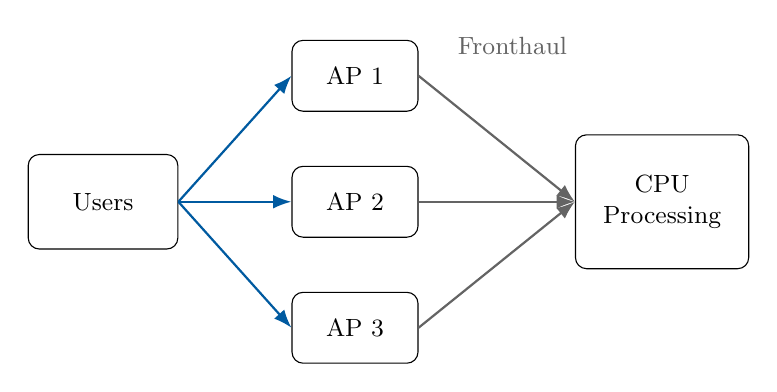
\begin{tikzpicture}[>=Latex,font=\small]
		\definecolor{ulcolor}{RGB}{0,90,160}
		\definecolor{fhcolor}{RGB}{100,100,100}
		
		\node[draw,rounded corners,minimum width=19mm,
		minimum height=12mm] (users) at (0,0) {Users};
		
		\foreach \q/\y in {1/1.6,2/0,3/-1.6}{
			\node[draw,rounded corners,minimum width=16mm,
			minimum height=9mm] (ap\q) at (3.2,\y) {AP $\q$};
			\draw[->,ulcolor,thick] (users.east) -- (ap\q.west);
		}
		
		\node[draw,rounded corners,minimum width=22mm,
		minimum height=17mm,align=center] (cpu) at (7.1,0)
		{CPU\\Processing};
		
		\foreach \q in {1,2,3}{
			\draw[->,fhcolor,thick] (ap\q.east) -- (cpu.west);
		}
		
		\node[above,text=fhcolor] at (5.2,1.75) {Fronthaul};
	\end{tikzpicture}
	\caption{Distributed uplink reception with $Q$ cooperating APs (three illustrated). Local observations or processed signals are transferred to a CPU through fronthaul connections.}
	\label{fig:distributed-05}
\end{figure}
\figref{fig:distributed-05} illustrates the logical processing architecture. The available fronthaul and local processing determine whether raw observations, combined signals, or decoded information are exchanged.

\subsection{Distributed channel properties and performance}
A simplified distributed fading model is
\begin{equation*}
	\ma h_{q,u}\sim
	\CNormal(\ma 0,\beta_{q,u}\ma I_{N_{\mathsf r,q}}),
\end{equation*}
with independent channels across APs and users. The coefficient $\beta_{q,u}$ represents the average channel gain between user $u$ and AP $q$. The aggregate channel covariance is
\begin{equation}
	\ma C_{h_u}
	=\diag{\beta_{1,u}\ma I_{N_{\mathsf r,1}},
		\ldots,\beta_{Q,u}\ma I_{N_{\mathsf r,Q}}},
	\qquad
	\Ex{\NormTwo{\ma h_u}^2}
	=\sum_{q=1}^{Q}N_{\mathsf r,q}\beta_{q,u}.
	\label{eq:distributedcov-05}
\end{equation}

Using the statistical diagnostics of Section~\ref{sec:statistics-05}, the relative channel-energy variance becomes
\begin{equation}
	\frac{\Var{\NormTwo{\ma h_u}^2}}
	{\Ex{\NormTwo{\ma h_u}^2}^2}
	=\frac{\displaystyle\sum_{q=1}^{Q}
		N_{\mathsf r,q}\beta_{q,u}^2}
	{\left(\displaystyle\sum_{q=1}^{Q}
		N_{\mathsf r,q}\beta_{q,u}\right)^2},
	\label{eq:distributedhard-05}
\end{equation}
while the normalized covariance overlap between users $i$ and $j$ is
\begin{equation}
	\frac{\Ex{|\mH{\ma h}_i\ma h_j|^2}}
	{\Ex{\NormTwo{\ma h_i}^2}\Ex{\NormTwo{\ma h_j}^2}}
	=\frac{\displaystyle\sum_{q=1}^{Q}
		N_{\mathsf r,q}\beta_{q,i}\beta_{q,j}}
	{\left(\displaystyle\sum_{q=1}^{Q}N_{\mathsf r,q}\beta_{q,i}\right)
		\left(\displaystyle\sum_{q=1}^{Q}N_{\mathsf r,q}\beta_{q,j}\right)}.
	\label{eq:distributedoverlap-05}
\end{equation}
Users served predominantly by different APs may have reduced channel overlap and improved spatial separability. However, if only a few ports contribute most of the received energy, channel hardening may be weaker than in a collocated system with more uniform channel gains.

\begin{example}{Equal aggregate gain with different spatial power distribution}
	Consider two users and two aggregate receive ports with independent Gaussian small-scale fading. A collocated reference has $\ma C_{h_1}=\ma C_{h_2}=0.55\ma I_2$, whereas a distributed reference has
	\begin{equation*}
		\ma C_{h_1}=\diag{1,0.1},
		\qquad
		\ma C_{h_2}=\diag{0.1,1}.
	\end{equation*}
	Both systems have the same number of ports and mean channel energy $1.1$ per user. The normalized covariance overlap decreases from $0.5$ to $0.2/1.21\approx0.165$, while the relative channel-energy variance increases from $0.5$ to $1.01/1.21\approx0.835$. Thus, distribution can improve statistical user separation while reducing channel hardening. These measures do not, by themselves, establish an achievable-rate ordering.
\end{example}

Beyond these statistical properties, geographical distribution provides macro-diversity against local shadowing and blockage. Users may retain useful links to other APs when one link becomes weak. These benefits depend on the spatial variability of the large-scale gains and the availability of cooperative processing.

\subsection{Centralized and distributed processing}
Although the aggregate model in \eqref{eq:distributed-ul-05} is identical to the collocated model, the feasible combining methods depend on where processing is performed and which information is exchanged.

\paragraph{Centralized combining.}
When the CPU receives all local samples and the required channel information, the aggregate combining matrix $\ma W\in\compl^{\NR\times U}$ can be designed jointly. The estimate is
\begin{equation*}
	\widehat{\ma x}=\mH{\ma W}\ma y.
\end{equation*}
The MRC, ZF, and LMMSE methods of Lecture~04 can then be applied to the aggregate channel. However, transporting the received samples and CSI from all APs requires fronthaul capacity and sufficiently accurate synchronization.

\paragraph{Local combining and CPU fusion.}
To reduce fronthaul requirements, the received samples may first be combined at the APs. For user $u$, AP $q$ produces
\begin{equation}
	r_{q,u}=\mH{\ma w}_{q,u}\ma y_q,
	\qquad
	\ma w_{q,u}\in\compl^{N_{\mathsf r,q}\times1}.
	\label{eq:localcombining-05}
\end{equation}
The local outputs are transferred to the CPU and combined using coefficients $a_{q,u}$:
\begin{equation}
	\widehat x_u=\sum_{q=1}^{Q}a_{q,u}^*r_{q,u},
	\qquad
	\ma w_u=
	\begin{bmatrix}
		a_{1,u}\ma w_{1,u}\\
		\vdots\\
		a_{Q,u}\ma w_{Q,u}
	\end{bmatrix}
	\in\compl^{\NR\times1}.
	\label{eq:twostage-05}
\end{equation}
The resulting estimate still has the form $\widehat x_u=\mH{\ma w}_u\ma y$, so the general SINR formulation remains applicable.

The difference lies in the information available for designing $\ma w_{q,u}$ and $a_{q,u}$. Local combining can use local CSI, while CPU fusion may use large-scale channel statistics or additional exchanged information. Without sufficiently detailed global CSI and observations, the fully centralized combining solution may not be realizable. The restriction arises from the available information and processing, rather than from the mathematical partition of $\ma w_u$ alone.

Centralized processing offers greater joint optimization freedom but requires more fronthaul resources. Local processing reduces the amount of transferred data, at the cost of restricted subsequent processing and possible performance loss. Fronthaul quantization, delay, and synchronization may introduce further limitations.

\paragraph{Distributed downlink precoding.}
In the DL, AP $q$ has $N_{\mathsf t,q}$ effective transmit ports, with
\begin{equation*}
	\NT=\sum_{q=1}^{Q}N_{\mathsf t,q}.
\end{equation*}
The BS precoder is partitioned into local matrices $\ma F_q\in\compl^{N_{\mathsf t,q}\times U}$, while the DL channel-column matrix is partitioned into $\ma H_q^{\mathsf{DL}}\in\compl^{N_{\mathsf t,q}\times U}$. The aggregate received signal is
\begin{equation}
	\boxed{
		\ma y=\sum_{q=1}^{Q}
		\mT{\ma H}_{\mathsf{DL},q}\ma F_q\ma d+\ma v
		=\mT{\ma H}_{\mathsf{DL}}\ma F\ma d+\ma v.
	}
	\label{eq:distributed-dl-05}
\end{equation}
The same transpose-based DL model is recovered, but precoder design must also account for the energy available at each AP. With $\ma R_d=\Ed\ma I_U$, the local energy constraint is
\begin{equation}
	\Ed\frob{\ma F_q}^2\leq E_q^{\mathsf{max}},
	\label{eq:apenergy-05}
\end{equation}
where $E_q^{\mathsf{max}}$ is the available transmit energy per channel use at AP $q$. These local constraints cannot generally be replaced by one aggregate constraint without changing the feasible precoders.

Coherent joint transmission requires accurate relative timing and carrier-phase alignment between cooperating APs, as well as suitable CSIT and distribution of user data. These requirements are more demanding than the aggregate digital signal model alone suggests.

\subsection{Cell-free operation and user-centric cooperation}
In cell-free massive MIMO, geographically distributed APs cooperate to serve users without assigning each user exclusively to a conventional fixed cell. A user-centric architecture selects a serving set $\mathcal Q_u\subseteq\{1,\ldots,Q\}$ for user $u$. APs outside this set do not contribute to that user's combining or precoding.

Such clustering limits the number of APs participating in each user's processing and can reduce CSI exchange, fronthaul traffic, and computation. Serving sets may overlap, allowing cooperation between APs while avoiding full network-wide processing. The design must balance cooperation gains against coordination and implementation costs. \Ac{comp} also involves coordination across transmission sites, but does not specify the same user-centric organization or processing architecture.

\begin{table}[htbp]
	\centering
	\small
	\caption{Comparison of multiuser MIMO deployment architectures.}
	\label{tab:architectures-05}
	\begin{tabular}{p{30mm}p{43mm}p{66mm}}
		\toprule
		Architecture & Main benefit & Main challenge\\
		\midrule
		Collocated MU-MIMO
		& Centralized processing and coordination
		& Limited spatial dimensions and site-dependent propagation\\
		Collocated massive MIMO
		& Array gain and spatial multiplexing with many ports
		& CSI acquisition and hardware/processing complexity\\
		Distributed/cell-free MIMO
		& User proximity, macro-diversity, and improved coverage
		& Fronthaul, synchronization, CSI sharing, and distributed processing\\
		\bottomrule
	\end{tabular}
\end{table}
\tabref{tab:architectures-05} summarizes the main architectural tradeoffs. Distribution can improve coverage, user separability, and fairness, but requires additional coordination and infrastructure. Its benefits depend on AP placement, channel conditions, energy allocation, and processing constraints. The common digital MU-MIMO model enables a consistent comparison without implying that one architecture is universally superior.


\section*{Summary and Outlook}
The main principles of massive and distributed multiuser MIMO are summarized as follows:
\begin{itemize}
	\item \textbf{Spatial dimensions and user loading:} Increasing the number of BS ports can improve channel gain and user separation. The available spatial dimensions depend on channel rank and conditioning, not merely on port count.
	
	\item \textbf{Favorable propagation and channel hardening:} Favorable propagation describes asymptotic orthogonality between user channels, whereas channel hardening describes decreasing relative channel-gain fluctuations. Neither property is guaranteed by increasing the port count alone.
	
	\item \textbf{Performance and energy scaling:} Massive MIMO can improve SINR or reduce transmit energy under suitable propagation and CSI assumptions. The gains depend on user loading and energy constraints, which differ between UL and DL. Instantaneous SINR, mean-power SINR ratios, and ergodic rates must be distinguished.
	
	\item \textbf{CSI acquisition and imperfections:} Pilot overhead, channel estimation errors, reciprocity calibration, and channel aging limit practical performance. Increasing the number of ports does not eliminate these constraints.
	
	\item \textbf{Distributed and cell-free MIMO:} Aggregating distributed antenna ports preserves the digital MU-MIMO model while changing channel statistics and processing constraints. User proximity, spatial diversity, and coverage may improve, but fronthaul, synchronization, and local energy constraints introduce additional challenges.
\end{itemize}

Lectures~01--05 established the digital MIMO framework and its performance under different channel and processing assumptions. Lecture~06 consolidates these principles through complementary examples and exercises. Part~II then examines how physical antenna arrays, propagation geometry, and analog frontend processing determine the effective digital channels used throughout Part~I.


\section*{Further reading}
\begin{thebibliography}{9}
\bibitem{massive} E.~Bj\"ornson, J.~Hoydis, and L.~Sanguinetti, \emph{Massive MIMO Networks: Spectral, Energy, and Hardware Efficiency}, 2017. Authors' book page: \url{https://massivemimobook.com/wp/}.
\bibitem{unlimited} E.~Bj\"ornson, J.~Hoydis, and L.~Sanguinetti, ``Massive MIMO Has Unlimited Capacity,'' \emph{IEEE Transactions on Wireless Communications}, 2018. Authors' manuscript: \url{https://arxiv.org/abs/1705.00538}.
\bibitem{cellfree} \"O.~T.~Demir, E.~Bj\"ornson, and L.~Sanguinetti, \emph{Foundations of User-Centric Cell-Free Massive MIMO}, 2021. Authors' manuscript: \url{https://arxiv.org/abs/2108.02541}.
\end{thebibliography}
\appendix
\clearpage

\section*{Review questions}
\begin{enumerate}[label=\textbf{E\arabic*.}]
	\item A BS has $\NR=64$ receive ports and serves $U=8$ users. Does this guarantee full user-channel rank? Determine the UL loading factor.
	
	\item Under independent Rayleigh fading, calculate the relative standard deviation of the channel energy for $\NR=25$ and $\NR=100$.
	
	\item For $\NR=64$, $U=8$, and $E_u=\beta_u=\sigma_v^2=1$, calculate the MRC mean-power SINR ratio and the mean ZF SINR. Why does neither quantity directly determine the exact ergodic rate?
	
	\item Under independent Rayleigh fading, fixed $U$, and perfect CSI, what happens to the UL MRC SINR when $E_u=\mathcal E_u/\NR$? What additional limitation arises if the pilot energy is also reduced?
	
	\item A coherence block contains $M=200$ channel uses and $U=40$ users requiring orthogonal pilots. Determine the minimum number of pilot uses $M_{\mathsf c}$ and the maximum data fraction, ignoring other overhead.
	
	\item Why is propagation reciprocity alone insufficient to determine the complete DL digital channel when $\NT\ne\NR$?
	
	\item A distributed system has $Q=2$ APs with $N_{\mathsf r,1}=2$ and $N_{\mathsf r,2}=3$ receive ports, serving $U=4$ users. Determine the dimensions of the local and aggregate UL channel matrices. What rank condition is required for four-user ZF combining?
	
	\item Explain why distributed antenna deployment can reduce covariance overlap between users while weakening channel hardening.
\end{enumerate}

\clearpage
\subsection*{Answers}
\begin{enumerate}[label=\textbf{E\arabic*.}]
	\item No. Full user rank depends on the channel vectors, not only the number of ports. The loading factor is $\zeta_{\mathsf{UL}}=U/\NR=8/64=1/8$. Full-column-rank ZF requires $\RH=8$.
	
	\item The relative standard deviation is $1/\sqrt{\NR}$, giving $0.2$ for $\NR=25$ and $0.1$ for $\NR=100$.
	
	\item The MRC mean-power SINR ratio is $\widetilde\gamma_u^{\mathsf{UL},\MRC}=64/(7+1)=8$, while the exact mean ZF SINR is $\Ex{\gamma_u^{\mathsf{UL},\ZF}}=64-8+1=57$. The first is a ratio of mean powers, not generally the mean SINR. The ergodic rate requires $\Ex{\log_2(1+\gamma_u)}$, which cannot generally be obtained by inserting either quantity into the logarithm.
	
	\item The MRC SINR converges in probability to $\mathcal E_u\beta_u/\sigma_v^2$. If the pilot energy also decreases, channel estimation quality may deteriorate, so the perfect-CSI scaling result need not remain valid.
	
	\item At least $M_{\mathsf c}=U=40$ pilot uses are required. The maximum data allocation is $M_{\mathsf d}=160$, corresponding to a fraction $M_{\mathsf d}/M=0.8$.
	
	\item Reciprocity relates propagation between corresponding physical ports. The effective digital channels also depend on RF hardware, calibration, and frontend processing. Different port configurations may include DL channel dimensions not observed during UL training.
	
	\item The local channel matrices have dimensions $\ma H_1\in\compl^{2\times4}$ and $\ma H_2\in\compl^{3\times4}$. Their aggregate channel is $\ma H\in\compl^{5\times4}$. Four-user ZF combining requires $\RH=U=4$.
	
	\item Different users may have strong channels to different APs, reducing covariance overlap and improving statistical user separation. However, each user may receive most of its energy through only a few strong channel components, increasing relative channel-energy fluctuations and weakening hardening.
\end{enumerate}


% ============================================================
\clearpage

\section{Gaussian channel moments and Gram-matrix convergence}
\label{app:moments-05}

Let $\ma h\sim\CNormal(\ma 0,\ma C_h)$, where $\ma C_h\in\compl^{n\times n}$ is Hermitian positive semidefinite. Using the eigenvalue decomposition $\ma C_h=\ma U\diag{\lambda_1,\ldots,\lambda_n}\mH{\ma U}$, the channel can be represented as $\ma h=\ma U\diag{\sqrt{\lambda_1},\ldots,\sqrt{\lambda_n}}\ma g$, with $\ma g\sim\CNormal(\ma 0,\ma I_n)$. Since $\Ex{|g_k|^2}=\Var{|g_k|^2}=1$, the channel-energy moments are
\begin{equation}
	\begin{split}
		\Ex{\NormTwo{\ma h}^2}
		&=\sum_{k=1}^{n}\lambda_k=\trace{\ma C_h},\\
		\Var{\NormTwo{\ma h}^2}
		&=\sum_{k=1}^{n}\lambda_k^2=\trace{\ma C_h^2}.
	\end{split}
\end{equation}
For independent zero-mean user channels $\ma h_i$ and $\ma h_j$,
\begin{equation}
	\begin{split}
		\Ex{|\mH{\ma h}_i\ma h_j|^2}
		&=\Ex{\mH{\ma h}_i\ma h_j\mH{\ma h}_j\ma h_i}\\
		&=\Ex{\mH{\ma h}_i\ma C_{h_j}\ma h_i}\\
		&=\trace{\ma C_{h_i}\ma C_{h_j}}.
	\end{split}
\end{equation}
These identities establish \eqref{eq:corrhard-05} and \eqref{eq:overlap-05}.

Under independent Rayleigh fading, $\ma C_{h_u}=\beta_u\ma I_{\NR}$, giving
\begin{equation*}
	\frac{\Var{\NormTwo{\ma h_u}^2}}
	{\Ex{\NormTwo{\ma h_u}^2}^2}
	=\frac{1}{\NR},
	\qquad
	\frac{\Ex{|\mH{\ma h}_i\ma h_j|^2}}
	{\Ex{\NormTwo{\ma h_i}^2}\Ex{\NormTwo{\ma h_j}^2}}
	=\frac{1}{\NR}.
\end{equation*}
For fixed $U$, the strong law of large numbers applied to the independent channel components gives the almost-sure convergence of the normalized Gram matrix in \eqref{eq:gramlimit-05}. This conclusion does not directly extend to a growing number of users without additional conditions.


\section{MRC SINR statistics and mean-power ratio}
\label{app:mrc-05}

For independent Rayleigh channels, the unit-norm MRC combiner $\ma w_u=\ma h_u/\NormTwo{\ma h_u}$ is independent of the interfering channels. Conditional on $\ma w_u$, the projections satisfy $\mH{\ma w}_u\ma h_j\sim\CNormal(0,\beta_j)$. Their squared magnitudes can therefore be represented by independent unit-mean exponential variables $V_j$, independent of $Z=\NormTwo{\ma h_u}^2$. The instantaneous SINR has the distribution
\begin{equation}
	\gamma_u^{\mathsf{UL},\MRC}
	\overset{\mathsf d}{=}
	\frac{E_u Z}{D},
	\qquad
	D=\sigma_v^2+\sum_{j\ne u}E_j\beta_jV_j,
	\qquad
	\frac{Z}{\beta_u}\sim\operatorname{Gamma}(\NR,1).
	\label{eq:mrcdistribution-05}
\end{equation}

Since $Z$ and $D$ are independent, the mean SINR and mean-power SINR ratio are
\begin{equation}
	\Ex{\gamma_u^{\mathsf{UL},\MRC}}
	=E_u\NR\beta_u\Ex{D^{-1}},
	\qquad
	\widetilde\gamma_u^{\mathsf{UL},\MRC}
	=\frac{E_u\NR\beta_u}{\Ex{D}}.
\end{equation}
By Jensen's inequality, $\Ex{D^{-1}}\geq1/\Ex{D}$, giving
\begin{equation}
	\boxed{
		\Ex{\gamma_u^{\mathsf{UL},\MRC}}
		\geq\widetilde\gamma_u^{\mathsf{UL},\MRC}.
	}
\end{equation}
This inequality applies to mean SINR and does not directly establish an ordering of achievable rates.

For fixed $U$ and user energies, the interference term in $D$ remains random as $\NR$ increases. If $E_u=\mathcal E_u/\NR$ for all users, then $D\to\sigma_v^2$ and $Z/\NR\to\beta_u$ in probability, yielding the MRC limit in \eqref{eq:energyscale-05}.

For equal user energies and gains with $U/\NR\to\zeta>0$, the law of large numbers gives
\begin{equation*}
	\frac{1}{\NR}\sum_{j\ne u}V_j\xrightarrow{\mathrm p}\zeta.
\end{equation*}
Substitution into \eqref{eq:mrcdistribution-05} gives $\gamma_u^{\mathsf{UL},\MRC}\xrightarrow{\mathrm p}1/\zeta$ for fixed per-user energy, as established in Section~\ref{sec:performance-05}.



\section{ZF projected gain and excess spatial dimensions}

Under independent Rayleigh fading with $\NR\geq U$, the channel matrix has full column rank almost surely. Let $\ma H_{-u}\in\compl^{\NR\times(U-1)}$ contain the channels of all users except $u$. The orthogonal projector onto their null space is
\begin{equation*}
	\ma\Pi_{-u}^{\perp}
	=\ma I_{\NR}
	-\ma H_{-u}\inv{(\mH{\ma H}_{-u}\ma H_{-u})}\mH{\ma H}_{-u},
\end{equation*}
with rank $k=\NR-U+1$. Since $\ma h_u$ is independent of $\ma\Pi_{-u}^{\perp}$, the ZF SINR can be expressed as
\begin{equation}
	\gamma_u^{\mathsf{UL},\ZF}
	=\frac{E_u}{\sigma_v^2}
	\mH{\ma h}_u\ma\Pi_{-u}^{\perp}\ma h_u,
	\qquad
	\frac{\sigma_v^2\gamma_u^{\mathsf{UL},\ZF}}{E_u\beta_u}
	\sim\operatorname{Gamma}(k,1).
\end{equation}
Consequently,
\begin{equation*}
	\Ex{\gamma_u^{\mathsf{UL},\ZF}}
	=\frac{E_u\beta_u}{\sigma_v^2}(\NR-U+1),
\end{equation*}
which proves \eqref{eq:zfmean-05}. For $k>1$, the inverse Gamma moment gives
\begin{equation*}
	\Ex{[\inv{(\mH{\ma H}\ma H)}]_{uu}}
	=\frac{1}{\beta_u(k-1)}
	=\frac{1}{\beta_u(\NR-U)}.
\end{equation*}
At $k=1$, this inverse moment diverges, although the mean ZF SINR remains finite.

For fixed $U$ and $E_u=\mathcal E_u/\NR$, the normalized projected gain satisfies
\begin{equation*}
	\Ex{\frac{\mH{\ma h}_u\ma\Pi_{-u}^{\perp}\ma h_u}{\NR}}
	=\frac{\beta_u k}{\NR}\longrightarrow\beta_u,
	\qquad
	\Var{\frac{\mH{\ma h}_u\ma\Pi_{-u}^{\perp}\ma h_u}{\NR}}
	=\frac{\beta_u^2 k}{\NR^2}\longrightarrow0.
\end{equation*}
This establishes the ZF limit in \eqref{eq:energyscale-05}. For $U/\NR\to\zeta\in(0,1)$, the projected dimension satisfies $k/\NR\to1-\zeta$, yielding the joint-loading behavior in \eqref{eq:jointscaling-05}.


\section{Additional scaling and channel-aging models}
\label{app:extensions-05}

\subsection{Fixed total uplink energy under joint loading}
Consider independent Rayleigh fading with equal large-scale gains $\beta_u=\beta$, perfect CSI, and $U/\NR\to\zeta\in(0,1)$. Under a fixed total UL data-energy budget $E_{\mathsf{sum}}$, each user transmits with $E_u=E_{\mathsf{sum}}/U$. The limiting SINRs are
\begin{equation}
	\begin{split}
		\gamma_u^{\mathsf{UL},\MRC}
		&\xrightarrow{\mathrm p}
		\frac{E_{\mathsf{sum}}\beta}
		{\zeta(E_{\mathsf{sum}}\beta+\sigma_v^2)},\\
		\gamma_u^{\mathsf{UL},\ZF}
		&\xrightarrow{\mathrm p}
		\frac{E_{\mathsf{sum}}\beta(1-\zeta)}
		{\zeta\sigma_v^2}.
	\end{split}
\end{equation}
This fixed-sum-energy constraint differs from the independent per-user energy assumptions in the basic UL model.

\subsection{A covariance-preserving channel-aging model}
A simple stationary Gaussian channel-aging model is
\begin{equation}
	\ma h_u[t+\Delta]
	=a_u(\Delta)\ma h_u[t]
	+\sqrt{1-|a_u(\Delta)|^2}\,\ma g_u,
\end{equation}
where $|a_u(\Delta)|\leq1$, $\ma h_u[t],\ma g_u\in\compl^{\NR\times1}$ are independent, and both follow $\CNormal(\ma0,\ma C_{h_u})$. The delay $\Delta$ is measured in symbol intervals. The model satisfies
\begin{equation*}
	\Ex{\ma h_u[t+\Delta]\mH{\ma h}_u[t+\Delta]}
	=\ma C_{h_u},
	\qquad
	\Ex{\ma h_u[t+\Delta]\mH{\ma h}_u[t]}
	=a_u(\Delta)\ma C_{h_u}.
\end{equation*}
Thus, the channel covariance is preserved while its correlation with the previous channel depends on $a_u(\Delta)$. The model illustrates CSI aging without specifying a particular mobility or oscillator process.


\section{Law of large numbers and channel convergence}
\label{app:lln-05}

The \textbf{law of large numbers (LLN)} describes the convergence of sample averages to their statistical means. For independent and identically distributed (i.i.d.) random variables $X_n$ with finite mean $\mu=\Ex{X_n}$, consider
\begin{equation*}
	\overline X_N=\frac{1}{N}\sum_{n=1}^{N}X_n.
\end{equation*}
The weak and strong laws establish different modes of convergence:
\begin{equation}
	\boxed{
		\underbrace{\overline X_N\xrightarrow[N\to\infty]{\mathrm p}\mu}_{\text{Weak law}},
		\qquad
		\underbrace{\overline X_N\xrightarrow[N\to\infty]{\mathrm{a.s.}}\mu}_{\text{Strong law}}.
	}
	\label{eq:lln-05}
\end{equation}
Convergence in probability means that the probability of a deviation larger than any fixed $\epsilon>0$ approaches zero. Almost-sure convergence means that the sample average converges to $\mu$ with probability one. Almost-sure convergence implies convergence in probability, but the converse does not generally hold.

For independent variables with common finite variance $\sigma_X^2$, the sample-average variance is $\Var{\overline X_N}=\sigma_X^2/N$. Chebyshev's inequality provides
\begin{equation}
	\Pr\left(|\overline X_N-\mu|\geq\epsilon\right)
	\leq\frac{\sigma_X^2}{N\epsilon^2}
	\xrightarrow[N\to\infty]{}0,
	\label{eq:llnchebyshev-05}
\end{equation}
which establishes the weak law under these assumptions. The strong law also holds for i.i.d. variables with finite absolute mean.

\textbf{Application to MIMO channels:} For independent Rayleigh fading with fixed $U$, the normalized Gram-matrix entries are averages of independent channel-component products:
\begin{equation}
	\frac{\mH{\ma h}_i\ma h_j}{\NR}
	=\frac{1}{\NR}\sum_{n=1}^{\NR}h_{n,i}^*h_{n,j}.
\end{equation}
Their means satisfy
\begin{equation*}
	\Ex{h_{n,i}^*h_{n,j}}
	=\begin{cases}
		\beta_i, & i=j,\\
		0, & i\ne j.
	\end{cases}
\end{equation*}
Applying the strong law to each fixed user pair gives
\begin{equation}
	\frac{\mH{\ma h}_i\ma h_j}{\NR}
	\xrightarrow[\NR\to\infty]{\mathrm{a.s.}}
	\beta_i\delta_{ij},
	\label{eq:llngram-05}
\end{equation}
establishing the normalized Gram-matrix limit in \eqref{eq:gramlimit-05}. The diagonal and off-diagonal limits correspond to channel hardening and favorable propagation, respectively. For growing $U$, entrywise convergence alone does not guarantee convergence of the entire Gram matrix in spectral norm.

\end{document}
